\documentclass{beamer}

\usetheme{Boadilla}

\usepackage{amsmath}
\usepackage[francais]{babel}
\usepackage[applemac]{inputenc}
\usepackage{tabularx}

\usepackage[boxed]{algorithm2e}
\usepackage{multimedia}
\usepackage{pgfpages}

\usenavigationsymbolstemplate{}

\setbeamertemplate{footline}[frame number,logo]
\defbeamertemplate{description item}{align left}{\insertdescriptionitem\hfill}

\title{DICOM II}
\subtitle{Cours HEdS Gen\`eve}
\author[B. Deville]{Beno\^it Deville - Analyste en informatique}
\institute[HUG]{H\^opitaux Universitaires de Gen\`eve}
\date{2016}

\begin{document}

\frame{\titlepage}

% outline
\section*{Plan}
\frame
{
  \frametitle{Plan}
  \tableofcontents
}

% repeat outline at each section
\AtBeginSection[] % Do nothing for \section*
{
      \begin{frame}<beamer>
         \frametitle{Rappel du plan}
         \tableofcontents[currentsection]
      \end{frame}
}

\section{Correction des exercices}

\frame
{
    \frametitle{Exercice 1}
	\begin{block}{\'Enonc\'e}
		Trouver l'ensemble des attributs obligatoires pour une IRM.
	\end{block}
}

\frame
{
    \frametitle{Exercice 2}
    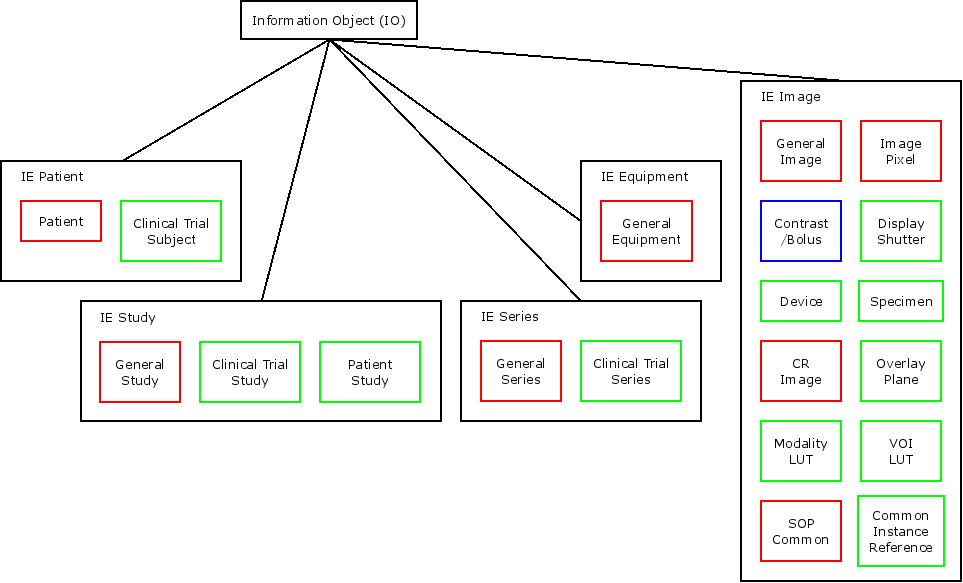
\includegraphics[width=\linewidth]{./figures/IO-definition-IE.png}

}

\frame
{
    \frametitle{Exercice 3}

    \begin{block}{Exercice}
        Jusqu'\`a combien pouvez-vous compter avec vos $10$ doigts ?
    \end{block}

    \begin{block}{R\'eponse}
        1023
    \end{block}

    \begin{center}
        
\includegraphics[width=.5\linewidth]{./figures/mains.png}
        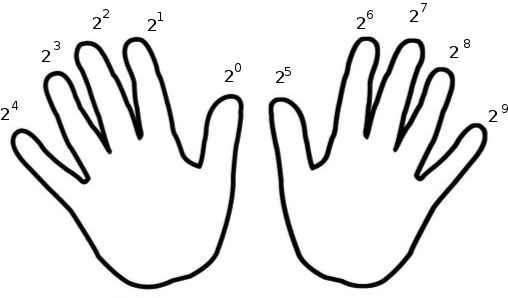
\includegraphics[width=.5\linewidth]{./figures/digits.png}
    \end{center}

}


\section{Rappels}

\frame
{
	\frametitle{Rappels}
	Vu au cours pr\'ec\'edent :
	\begin{itemize}
		\item Historique de DICOM.
		\item DICOM est un standard, pas une norme.
		\item DICOM d\'efinit des SOP (Service-Object Pair) :
		\begin{center}
			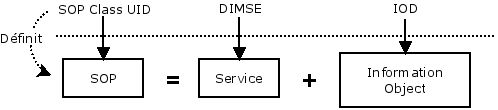
\includegraphics[width=\linewidth]{./figures/sop-definition.png}
		\end{center}
	\end{itemize}
}



\section{Repr\'esentations informatiques}

	\frame
	{
		\frametitle{Jeu de mains\ldots}
		
		\begin{block}{Exercice}
			Jusqu'\`a combien pouvez-vous compter avec vos $10$ doigts ?
		\end{block}
		
		\begin{block}{R\'eponse}
			1023 !
		\end{block}
		
		\begin{center}
			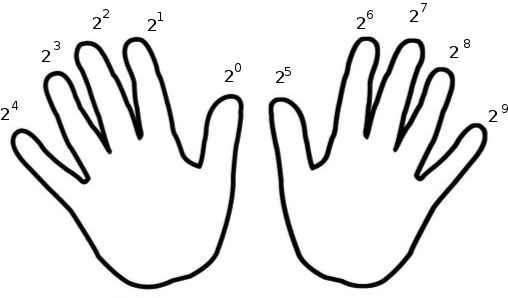
\includegraphics[width=.5\linewidth]{./figures/digits.png}
		\end{center}

	}
	
	\frame
	{
		\frametitle{Repr\'esentations num\'eriques}
		\begin{itemize}
			\item Repr\'esentation num\'erique : \emph{syst\`eme de num\'eration}.
			\item Syst\`eme de num\'eration connu, le \emph{d\'ecimal}, avec $10$ symboles :
				
			$0$ $1$ $2$ $3$ $4$ $5$ $6$ $7$ $8$ $9$
			\item Soit le nombre 1\textcolor{blue}{9}\textcolor{red}{9} :
			
			\textcolor{blue}{9}$~\neq~$\textcolor{red}{9}
			$\Rightarrow$ valeur d\'epend de la position : \emph{syst\`eme de num\'eration positionnel}.

			\item $0 \rightarrow 1\rightarrow  2 \rightarrow 3 \rightarrow 4 \rightarrow 5 \rightarrow 6 \rightarrow 7 \rightarrow 8 \rightarrow 9\rightarrow ?$ : on \emph{incr\'emente la position suivante} $\rightarrow 10$
			
			$10$ symboles $\Rightarrow$ \emph{base 10} : \emph{syst\`eme de num\'eration positionnel en base 10}.
		\end{itemize}
	}
	
	\frame
	{
		\frametitle{Notion de \emph{base}}
		
		Une repr\'esentation num\'erique doit \^etre adapt\'ee \`a ce qu'elle compte.
		\begin{itemize}
			\item Base $10$ : $10$ doigts.
			\item Autre base connue ;  $60$.
			\item \'Electronique (et par extention informatique) :
			\begin{itemize}
				\item base $2$,
				\item ou \emph{binaire},
				\item $0/1$, soit pas de courant/courant.
			\end{itemize}
			\item Informatique
			\begin{itemize}
				\item base $4$ (Bi-Binaire),
				\item base $8$ (octal),
				\item ou base $16$ (hexad\'ecimal) : 0 1 2 3 4 5 6 7 8 9 A($=10$) B($=11$) C($=12$) D($=13$) E($=14$) F($=15$).
			\end{itemize}
		\end{itemize}
	}
	
	\frame
	{
		\frametitle{G\'en\'eralisation}
		\begin{block}{D\'efinition}
			Soit $x$ un nombre \`a $n$ chiffres dans le syst\`eme de num\'eration positionnel en base $b$.
			
			Alors $x$ s'\'ecrit
			
			$x_{n-1}x_{n-2}\ldots x_1x_0$
			
			et $x=\sum\limits_{i = 0}^{n-1}x_i\cdot b^i$.
		\end{block}
		
		Exemples :
		\begin{description}
			\item $2013_{10} = 2\cdot10^3 + 0\cdot10^2 + 1\cdot10^1+3\cdot10^0$
			\item $199_{10} = 1\cdot2^7 + 1\cdot2^6 + 0\cdot2^5+0\cdot2^4 + 0\cdot2^3 + 1\cdot2^2 + 1\cdot2^1+1\cdot2^0 = 11000111_2$
		\end{description}
	}

\frame
{
	\frametitle{Little ou Big Endian}
	\begin{itemize}
		\item Origines chaotiques de l'informatique.
		\item Diff\'erents ordres de stockage pour les valeurs encod\'ees sur plusieurs octets (1 octet = 8 bits = $2^8$ possibilit\'es = 256 valeurs).
		\begin{itemize}
			\item Little Endian : moins importants en dernier.
			\item Big Endian : plus importants en dernier.
		\end{itemize}
		\item Exemple avec l'entier 2012 :
		\begin{itemize}
			\item Sur 2 octets
			\begin{itemize}
				\item Little Endian : 0x07DC
				\item Big Endian : 0xDC07
			\end{itemize}
			\item Sur 4 octets
			\begin{itemize}
				\item Little Endian : 0x000007DC
				\item Big Endian : 0xDC070000
			\end{itemize}
		\end{itemize}
	\end{itemize}
}


\section{Fichier DICOM}

\frame
{
	\frametitle{Conventions DICOM}
	\begin{itemize}
		\item Single Frame
		\begin{itemize}
			\item Une image : stock\'ee dans un fichier.
			\item Une coupe = une image
		
			$\Rightarrow$ s\'erie de 100 coupes = 100 fichiers.
		\end{itemize}
		\item Multiframe
		\begin{itemize}
			\item Aussi appel\'e \emph{Enhanced DICOM}.
			\item Plusieurs images dans la m\^eme s\'equence.
			
			E.g. s\'equence vid\'eo d'\'echographie.
		\end{itemize}
		\item Arborescence des r\'epertoires/fichiers
		\begin{center}
			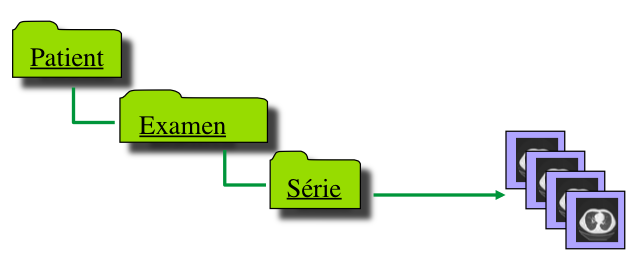
\includegraphics[width=.8\linewidth]{./figures/arborescence.png}
		\end{center}

	\end{itemize}
}

\frame
{
	\frametitle{Fichier en pratique}
	
	\begin{itemize}
		\item Peut \^etre exp\'edi\'e par messagerie.
		\item Convertible en d'autres formats (JPEG, AVI, etc.)
		\item Extenstion : .dcm
		\item Exemple avec OsiriX.
	\end{itemize}
}

\frame
{
	\frametitle{Contenu d'un fichier .dcm}
	
	Un fichier DICOM est l'agr\'egation des \'el\'ements suivants :
	\begin{itemize}
		\item Pr\'e-ent\^ete :
		\begin{itemize}
			\item Pr\'eambule : 128 octets de donn\'ees "application".
			\item Pr\'efixe : 0x4449434D=DICM (4 octets).
		\end{itemize}
		\item Suite de Data Elements.
		En g\'en\'eral :
		\begin{itemize}
			\item Tag ;
			\item VR ;
			\item Taille ;
			\item et Valeur.
		\end{itemize}
	\end{itemize}
}

\frame
{
	\frametitle{Tag}

	Il s'agit de l'\'etiquette d'identification d'un \'el\'ement d'information.
	\begin{itemize}
		\item Identifi\'e par un couple de deux nombres en h\'exad\'ecimal (Group Number, Element Number) :
			\begin{description}
				\item[Group Number] Identifiant d'un ensemble de tags (e.g. Patient, Study,\ldots).
				\item[Element Number] Position de l'\'el\'ement dans son groupe.
			\end{description}
		\item Exemple : l'\'el\'ement \emph{PatientID} a pour tag $(0010,0020)$.
		\item Une liste -- quasi -- exhaustive des tags ($3307$ tags diff\'erents, y compris nombre de tags obsol\`etes) : \url{http://www.dicomtags.com/iods}
		\item Certains tags sont "propri\'etaires", i.e. cr\'e\'es et utilis\'es par un constructeur particulier.
	\end{itemize}
}

\frame
{
	\frametitle{Value Representation}

	\begin{itemize}
		\item Tous les \'el\'ements ne sont pas repr\'esent\'es par le m\^eme type de donn\'ees.
		\item Donn\'ee num\'erique $\neq$ Donn\'ee textuelle.
		\item Ensemble des VR : \url{http://www.dicomtags.com/vrs}
	\end{itemize}
}


\section{Services DICOM}

\frame
{
	\frametitle{Services DICOM}
	
	\begin{itemize}
		\item \'Equivalent des IOD pour les services : DIMSE (DICOM Message Service Element).
		\item D\'efinir les op\'erations possibles selon les objets.
		\item Deux cat\'egories d'\'el\'ements :
		\begin{itemize}
			\item op\'erations (par exemple \emph{store}) ;
			\item notifications (e.g. \emph{event report}).
		\end{itemize}
		\item Services diff\'erents sur les objets composites ou normalis\'es :
		\begin{description}
			\item[Composites] C-STORE, C-FIND, C-MOVE, C-GET, C-ECHO.
			\item[Normalis\'es] N-GET, N-ACTION, N-SET, N-CREATE, N-DELETE, N-EVENT-REPORT.
			\item[Web] QIDO-RS, WADO-RS, WADO-URI, STOW-RS, UPS-RS, CAPABILITIES.
		\end{description}
	\end{itemize}
}

\frame
{
	\frametitle{Services principaux}
	\setbeamertemplate{description item}[align left]
	\begin{description}
		\item[Store] Envoi/stockage d'objets DICOM.
		\item[Storage Commitment] Confirmer l'archivage permanent d'une image.
		\item[Query/Retrieve]~\\
		\begin{itemize}
			\item Interrogation par crit\`eres \`a diff\'erents niveaux (e.g. patient, examen, s\'erie, image,).
			\item R\'ecup\'eration d'images/s\'eries/examens selon ces m\^emes crit\`eres.
		\end{itemize}
		\item[Modality worklist]~\\
		\begin{itemize}
			\item Interrogation par une modalit\'e du syst\`eme de planification.
			\item R\'ecup\'eration de la liste des examens pr\'evus.
			\item Examens document\'es : identification du patient, proc\'edure, prescripteur.
		\end{itemize}
		\item[MPPS] Diffuser l'information d'avancement d'un examen.
	\end{description}
}

\frame
{
	\frametitle{Communication}
	\begin{itemize}
		\item Chaque \'equipement joue un r\^ole d\'ependant du service :
		\begin{description}
			\item[SCU] Service Class User (le client).
			\item[SCP] Service Class Provider (le serveur).
		\end{description}
		\item Le SCU initie une demande, le SCP, qui fournit le service, r\'epond.
	\end{itemize}
	
	\begin{center}
		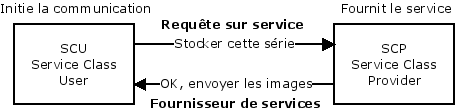
\includegraphics[width=.8\linewidth]{./figures/scu-scp.png}
	\end{center}
}

\frame
{
	\frametitle{Changement de r\^ole}
	Un \'equipement peut changer de r\^ole.
	
	Par exemple, une station d'interpr\'etation A peut \^etre :
	\begin{itemize}
		\item SCU dans un premier temps :
		\begin{enumerate}
			\item A sollicite un examen au PACS ;
			\item Le PACS accepte et envoie l'examen \`a A.
		\end{enumerate}
		\item puis SCP dans un second temps :
		\begin{enumerate}
		\setcounter{enumi}{2}
			\item B demande l'examen \`a A ;
			\item A transmet l'examen \`a B.
		\end{enumerate}
	\end{itemize}
	
	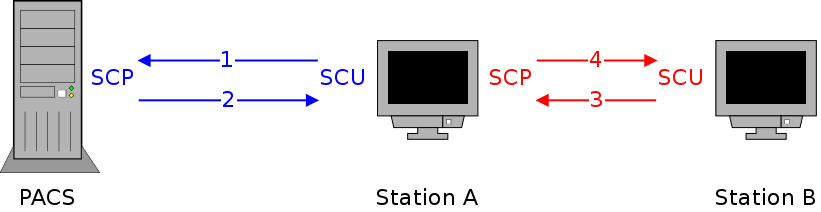
\includegraphics[width=\linewidth]{./figures/roles.png}
}


\section{DICOM en pratique}

\frame
{
	\frametitle{Anonymisation}
	\begin{itemize}
		\item Utilisation d'images cliniques pour la recherche ou l'enseignement.
		\item Fichiers mis \`a disposition du public.
		\item N\'ecessit\'e d'anonymat : suppression des informations personnelles permettant d'identifier le patient.
		\begin{itemize}
			\item PatientsName (0010,0010)
			\item PatientID (0010,0020)
			\item PatientBirthDate (0010,0030)
			
			$\rightarrow$ de type 1 : \`a remplacer, pas supprimer !
			\item ReferringPhysicianName (0008,0090)
			\item etc.
			\item Potentiellement plus de 250 champs \`a supprimer ou \`a vider !
		\end{itemize}
	\end{itemize}
}

\frame
{
	\frametitle{Achat d'un \'equipement}
	\begin{enumerate}
		\item Avant l'achat, soumission de l'appel d'offre :
		\begin{itemize}
			\item D\'efinition du sc\'enario de travail souhait\'e.

                Exemple : les images brutes export\'ees pourront \^etre r\'eutilis\'ees \emph{a posteriori}.
			\item R\'edaction du cahier des charges DICOM.
			\begin{itemize}
				\item Pr\'eciser le niveau d'exigence de DICOM.
				
				$\rightarrow$ faire appel \`a un consultant ou \`a des coll\`egues,
				
				$\rightarrow$ ou acqu\'erir le savoir-faire en interne.
				\item Demander le Document de Conformit\'e DICOM (DICOM Conformance Statement).
			\end{itemize}
		\end{itemize}
		\item Acceptation protocol\'ee.
		\begin{itemize}
			\item V\'erification de DICOM.
			\item V\'erification du/des sc\'enario/ii requis.
			\item Tests.
		\end{itemize}
	\end{enumerate}
}

\frame
{
	\frametitle{DICOM Conformance}
	\begin{itemize}
		\item Le standard pr\'evoit un document "DICOM Conformance Statement" dont le plan et la structure sont pr\'ed\'efinis.
		\item Par ce document, le fournisseur pr\'ecise le niveau de conformit\'e de son \'equipement au standard DICOM.
		\begin{itemize}
			\item Applicable sur chaque mod\`ele, chaque version.
			\item Le document suit un plan pr\'evu dans le standard.
			\item Liste des SOP Class support\'ees et des r\^oles assur\'es (SCU, SCP).
		\end{itemize}
	\end{itemize}
}

%\frame
%{
%	\frametitle{Exemple de DICOM Conformance Statement}
%}

\frame
{
	\frametitle{Services \`a demander}
	Exemples typiques de services DICOM \`a exiger pour un scanner :
	\begin{itemize}
		\item Worklist (SCU) : Import de la liste de patients.
		\item Store : envoi des images par r\'eseau
		\begin{itemize}
			\item Envoi : modalit\'es (SCU) : \textbf{CT}.
			\item R\'eception (SCP) : \textbf{CT}, \textbf{IRM}.
		\end{itemize}
		\item Print (SCU) : envoi des images pour impression
	\end{itemize}
	
	\begin{center}
		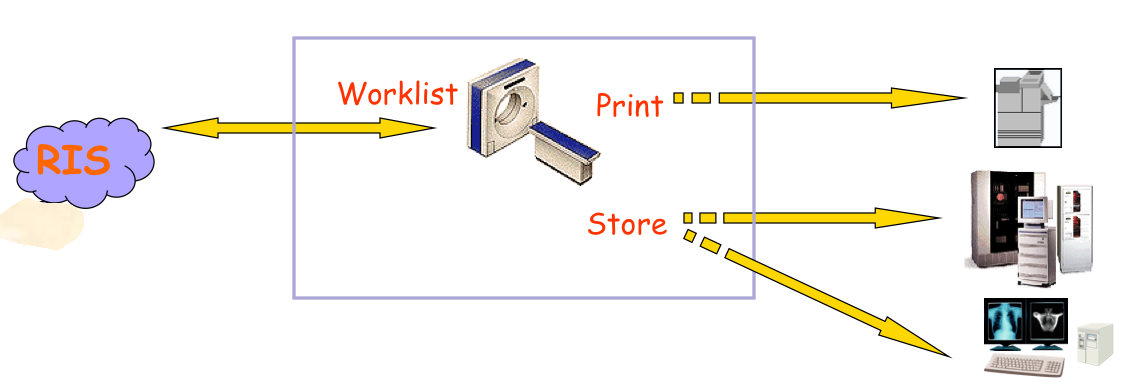
\includegraphics[width=\linewidth]{./figures/services-ct.png}
	\end{center}

}

\frame
{
	\frametitle{\'Equipements non standards}
	
	\begin{itemize}
		\item Int\'egrer dans un workflow DICOM : installer une passerelles de conversion.
		
		\begin{center}
			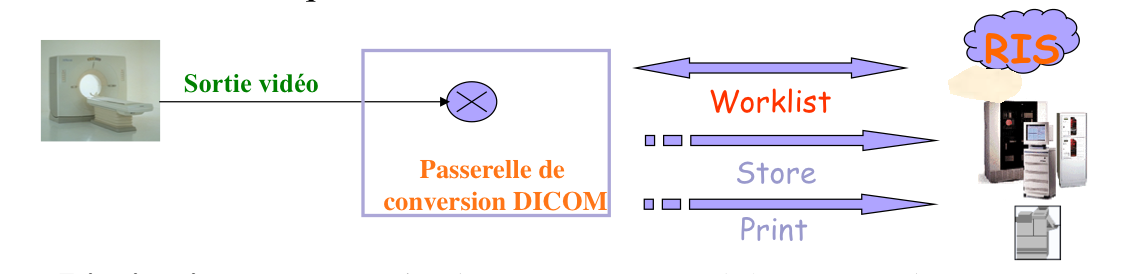
\includegraphics[width=\linewidth]{./figures/passerelle.png}
		\end{center}
		\item Limitation : images stock\'ees en mode Secondary Capture (IOD le plus simple de DICOM), les donn\'ees d'acquisition des images sont perdues.
	\end{itemize}
}


\section{Conclusions}

\frame
{
	\frametitle{Synth\`ese}
	
	\begin{itemize}
		\item Standard incontournable.
		\item Adopt\'e par la majorit\'e des acteurs (constructeurs, \'editeurs de logiciels, clients).
		\item Spectre plus large que l'imagerie radiologique.
		\item Conseil : pr\'evoir DICOM d\`es l'achat de l'\'equipement.
		\begin{itemize}
			\item M\^eme si l'export des images se fera plus tard.
			\item Surco\^ut restera inf\'erieur \`a l'achat d'options a posteriori.
		\end{itemize}
		\item Pr\'evoir plut\^ot que subir !
	\end{itemize}
}


%\section{Correction des exercices}

\frame
{
    \frametitle{Exercice 1}
	\begin{block}{\'Enonc\'e}
		Trouver l'ensemble des attributs obligatoires pour une IRM.
	\end{block}
}

\frame
{
    \frametitle{Exercice 2}
	\begin{block}{\'Enonc\'e}
		Faire un sch\'ema des \emph{Information Entities}, modules, et attributs obligatoires pour l'IOD \emph{Comprehensive SR}.
	\end{block}

}

%\frame
%{
%    \frametitle{Exercice 3}
%
%    \begin{block}{Exercice}
%        Jusqu'\`a combien pouvez-vous compter avec vos $10$ doigts ?
%    \end{block}
%
%    \begin{block}<2->{R\'eponse}
%        1023
%    \end{block}
%
%    \begin{center}
%        \includegraphics<3>[width=.5\linewidth]{./figures/mains.png}
%        \includegraphics<4>[width=.5\linewidth]{./figures/digits.png}
%    \end{center}
%
%}

%\section{Rappels}

\frame
{
	\frametitle{Notions abord�es au cours pr�c�dent}
	
	\begin{itemize}
		\item SOP = Service Object Pair.
		
		\begin{center}
			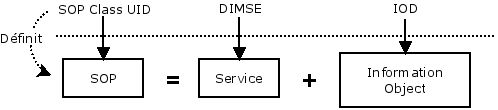
\includegraphics[width=.8\linewidth]{./figures/sop-definition.png}
		\end{center}
		
		Pour clarifier un peu : Object $\rightarrow$ \emph{Information Object} (\emph{IO}).
		
		\item Standard = annuaire.
		SOP Class UID vous permet de trouver � quel service et quel IOD il correspond.
		
		\item Attribut : une valeur.
		
		\item Module : ensemble d'attributs li�s.
		
		\item IOD = Information Object Definition.
		
		D�finit les modules (et donc les attributs) qui doivent �tre pr�sents pour un IO sp�cifique.
		
	\end{itemize}
}

\frame
{
	\frametitle{Information Object Defintion (IOD)}
	
	\begin{center}
	Ins�rer sch�ma de d�finition de l'IOD
%		\includegraphics[width=.8\linewidth]{./figures/iod-definition.png}
	\end{center}
}

%\section{Repr\'esentations informatiques}

	\frame
	{
		\frametitle{Repr\'esentations num\'eriques}
		\begin{itemize}
			\item<1-> Repr\'esentation num\'erique : \emph{syst\`eme de num\'eration}.
			\item<2-> Syst\`eme de num\'eration connu, le \emph{d\'ecimal}, avec $10$ symboles :
				
			$0$ $1$ $2$ $3$ $4$ $5$ $6$ $7$ $8$ $9$
			\item<3-> Soit le nombre 1\textcolor{blue}{9}\textcolor{red}{9} :
			
			\textcolor{blue}{9}$~\neq~$\textcolor{red}{9}
			$\Rightarrow$ valeur d\'epend de la position : \emph{syst\`eme de num\'eration positionnel}.

			\item<4-> $0 \rightarrow 1\rightarrow  2 \rightarrow 3 \rightarrow 4 \rightarrow 5 \rightarrow 6 \rightarrow 7 \rightarrow 8 \rightarrow 9\rightarrow ?$ : on \emph{incr\'emente la position suivante} $\rightarrow 10$
			
			$10$ symboles $\Rightarrow$ \emph{base 10} : \emph{syst\`eme de num\'eration positionnel en base 10}.
		\end{itemize}
	}
	
	\frame
	{
		\frametitle{Notion de \emph{base}}
		
		Une repr\'esentation num\'erique doit \^etre adapt\'ee \`a ce qu'elle compte.
		\begin{itemize}
			\item<2-> Base $10$ : $10$ doigts.
			\item<3-> Autre base connue :  $60$.
			\item<4-> \'Electronique (et par extension informatique) :
			\begin{itemize}
				\item<5-> base $2$,
				\item<6-> ou \emph{binaire},
				\item<7-> $1/0$, soit du courant/pas de courant.
			\end{itemize}
			\item<8-> Informatique
			\begin{itemize}
				\item<9-> base $4$ (Bi-Binaire),
				\item<10-> base $8$ (octal),
				\item<11-> ou base $16$ (hexad\'ecimal) : 0 1 2 3 4 5 6 7 8 9 A($=10$) B($=11$) C($=12$) D($=13$) E($=14$) F($=15$).
			\end{itemize}
		\end{itemize}
	}
	
	\frame
	{
		\frametitle{G\'en\'eralisation}
		\begin{block}{D\'efinition}
			Soit $x$ un nombre \`a $n$ chiffres dans le syst\`eme de num\'eration positionnel en base $b$.
			
			Alors $x$ s'\'ecrit
			
			$x_{n-1}x_{n-2}\ldots x_1x_0$
			
			et $x=\sum\limits_{i = 0}^{n-1}x_i\cdot b^i$.
		\end{block}
		
		Exemples :
		\begin{description}
			\item<2-> $2018_{10} = 2\cdot10^3 + 0\cdot10^2 + 1\cdot10^1+8\cdot10^0$
			\item<3-> $199_{10} = 1\cdot2^7 + 1\cdot2^6 + 0\cdot2^5+0\cdot2^4 + 0\cdot2^3 + 1\cdot2^2 + 1\cdot2^1+1\cdot2^0 = 11000111_2$
		\end{description}
	}

\frame
{
	\frametitle{Little ou Big Endian}
	\begin{itemize}
		\item<2-> Origines chaotiques de l'informatique.
		\item<3-> Diff\'erents ordres de stockage pour les valeurs encod\'ees sur plusieurs octets (1 octet = 8 bits = $2^8$ possibilit\'es = 256 valeurs).
		\begin{itemize}
			\item<4-> Little Endian : moins importants en dernier.
			\item<5-> Big Endian : plus importants en dernier.
		\end{itemize}
		\item<6-> Exemple avec l'entier 2018 :
		\begin{itemize}
			\item<7-> Sur 2 octets
			\begin{itemize}
				\item<8-> Little Endian : 0x07E2
				\item<9-> Big Endian : 0xE207
			\end{itemize}
			\item<10-> Sur 4 octets
			\begin{itemize}
				\item<11-> Little Endian : 0x000007E2
				\item<12-> Big Endian : 0xE2070000
			\end{itemize}
		\end{itemize}
	\end{itemize}
}

\frame
{
    \frametitle{Le rapport avec DICOM ?}
    \begin{itemize}
        \item Un Data Element contient 4 champs (Tag, Value Representation, Size, Value) dont :
        \begin{description}
            \item<2->[Tag] En h\'exad\'ecimal.
            \item<3->[VR] Le type d'encodage de la valeur.\\
                \includegraphics<4->[width=.5\linewidth]{./figures/types.jpg}
        \end{description}
        \item<5-> Certains DICOM cod\'es en Little Endian, d'autres en Big Endian. 
    \end{itemize}
}

\frame
{
    \frametitle{Types de VR}
    L'ensemble des VR existants est d\'efini dans la table 6.2-1 \emph{DICOM Value Representation} du chapitre 5 (\emph{Data Structures and Encoding}) du standard.

    Quelques exemples :
    \begin{description}
        \item<2->[AS] Age String (e.g. 023Y, 005M, 012D).
        \item<3->[DA] Date, au format YYYYMMDD.
        \item<4->[DT] Date Time, YYYYMMDDHHMMSS.FFFFFF\&{}ZZXX.
        \item<5->[OD] Other Double String (suite de $2^{32}$ octets maximum).
        \item<6->[PN] Person Name (e.g. Doe\^{}John).
        \item<7->[UI] Unique Identifier (UID), 64 caract\`eres maximum (\{0-9,.\}).
    \end{description}
}


%\section{Fichier DICOM}

\frame
{
	\frametitle{Conventions DICOM}
	\begin{itemize}
		\item Single Frame
		\begin{itemize}
			\item Une image : stock\'ee dans un fichier.
			\item Une coupe = une image
		
			$\Rightarrow$ s\'erie de 100 coupes = 100 fichiers.
		\end{itemize}
		\item Multiframe
		\begin{itemize}
			\item Aussi appel\'e \emph{Enhanced DICOM}.
			\item Plusieurs images dans la m\^eme s\'equence.
			
			E.g. s\'equence vid\'eo d'\'echographie.
		\end{itemize}
		\item Arborescence des r\'epertoires/fichiers
		\begin{center}
			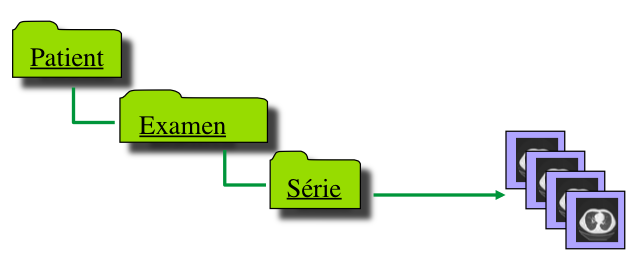
\includegraphics[width=.8\linewidth]{./figures/arborescence.png}
		\end{center}

	\end{itemize}
}

\frame
{
	\frametitle{Fichier en pratique}
	
	\begin{itemize}
		\item Peut \^etre exp\'edi\'e par messagerie.
		\item Convertible en d'autres formats (JPEG, AVI, etc.)
		\item Extenstion : .dcm
		\item Exemple avec OsiriX.
	\end{itemize}
}

\frame
{
	\frametitle{Contenu d'un fichier .dcm}
	
	Un fichier DICOM est l'agr\'egation des \'el\'ements suivants :
	\begin{itemize}
		\item Pr\'e-ent\^ete :
		\begin{itemize}
			\item Pr\'eambule : 128 octets de donn\'ees "application".
			\item Pr\'efixe : 0x4449434D=DICM (4 octets).
		\end{itemize}
		\item Suite de Data Elements.
		En g\'en\'eral :
		\begin{itemize}
			\item Tag ;
			\item VR ;
			\item Taille ;
			\item et Valeur.
		\end{itemize}
	\end{itemize}
}

%\section{Services DICOM}

\frame
{
	\frametitle{Services DICOM}
	
	\begin{itemize}
		\item<1-> \'Equivalent des IOD pour les services : DIMSE (DICOM Message Service Element).
		\item<2-> D\'efinir les op\'erations possibles selon les objets.
		\item<3-> Deux cat\'egories d'\'el\'ements :
		\begin{itemize}
			\item<4-> op\'erations (par exemple \emph{store}) ;
			\item<5-> notifications (e.g. \emph{event report}).
		\end{itemize}
		\item<6-> Services diff\'erents selon les objets
		\begin{description}
			\item<7->[Composites] C-STORE, C-FIND, C-MOVE, C-GET, C-ECHO.
			\item<8->[Normalis\'es] N-GET, N-ACTION, N-SET, N-CREATE, N-DELETE, N-EVENT-REPORT.
			\item<9->[Web] QIDO-RS, WADO-RS, WADO-URI, STOW-RS, UPS-RS, CAPABILITIES.
		\end{description}
	\end{itemize}
}

\frame
{
	\frametitle{Services principaux}
	\setbeamertemplate{description item}[align left]
	\begin{description}
		\item<2->[Store] Envoi/stockage d'objets DICOM.
		\item<3->[Storage Commitment] V\'erification de l'archivage d'une image.
		\item<4->[Query/Retrieve]~\\
		\begin{itemize}
			\item<5-> Interrogation par crit\`eres \`a diff\'erents niveaux (e.g. patient, examen, s\'erie, image) :
			\item<6-> R\'ecup\'eration d'images/s\'eries/examens selon ces m\^emes crit\`eres.
		\end{itemize}
		\item<7->[Modality worklist]~\\
		\begin{itemize}
			\item<8-> Interrogation par une modalit\'e du syst\`eme de planification.
			\item<9-> R\'ecup\'eration de la liste des examens pr\'evus.
			\item<10-> Examens document\'es (identito-vigilance) : identification du patient, proc\'edure, prescripteur.
		\end{itemize}
		\item<11->[MPPS] V\'ehiculer les informations sur ce qui est r\'ealis\'e par un syst\`eme.
	\end{description}
}

%\frame
%{
%	\frametitle{Autres services}
%	\setbeamertemplate{description item}[align left]
%	\begin{description}
%		\item<1->[Printing]~\\
%		D\'emod\'e depuis les imprimantes PostScript.
%		\item<2->[Storage commitment]~\\
%		Confirmer qu'un objet est stock\'e de mani\`ere permanente.
%		\item<3->[Modality performed procedure step]~\\
%		Permet de diffuser l'information d'avancement d'un examen.
%		\item<4->[Offline media]~\\
%		D\'etails sur le stockage sur support CD, DVD, etc.
%	\end{description}
%}

\frame
{
	\frametitle{Communication}
	\begin{itemize}
		\item Chaque \'equipement joue un r\^ole d\'ependant du service :
		\begin{description}
			\item<2->[SCU] Service Class User (le client).
			\item<3->[SCP] Service Class Provider (le serveur).
		\end{description}
		\item<4-> Le SCU initie une demande, le SCP, qui fournit le service, r\'epond.
	\end{itemize}
	
	\begin{center}
		\includegraphics<5->[width=.8\linewidth]{./figures/scu-scp.png}
	\end{center}
}

\frame
{
	\frametitle{Changement de r\^ole}
	Un \'equipement peut changer de r\^ole.
	
	Par exemple, une station d'interpr\'etation A peut \^etre :
	\begin{itemize}
		\item<2-> SCU dans un premier temps :
		\begin{enumerate}
			\item<3-> A sollicite un examen au PACS ;
			\item<4-> Le PACS accepte et envoie l'examen \`a A.
		\end{enumerate}
		\item<5-> puis SCP dans un second temps :
		\begin{enumerate}
		\setcounter{enumi}{2}
			\item<6-> B demande l'examen \`a A ;
			\item<7-> A transmet l'examen \`a B.
		\end{enumerate}
	\end{itemize}
	
%	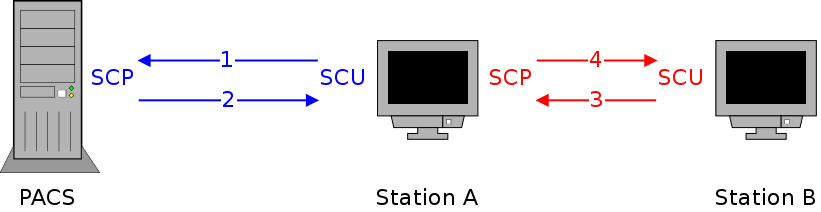
\includegraphics[width=\linewidth]{./figures/roles.png}
	\includegraphics<2>[width=.6\linewidth]{./figures/roles-scu.png}
	\includegraphics<3>[width=.6\linewidth]{./figures/roles-1.png}
	\includegraphics<4>[width=.6\linewidth]{./figures/roles-2.png}
	\includegraphics<5>[width=\linewidth]{./figures/roles-scp.png}
	\includegraphics<6>[width=\linewidth]{./figures/roles-3.png}
	\includegraphics<7>[width=\linewidth]{./figures/roles-4.png}
}

%\section{DICOM en pratique}

\frame
{
	\frametitle{Anonymisation}
	\begin{itemize}
		\item<1-> Utilisation d'images cliniques pour la recherche ou l'enseignement.
		\item<2-> Fichiers mis \`a disposition du public.
		\item<3-> N\'ecessit\'e d'anonymat : suppression des informations personnelles permettant d'identifier le patient.
		\begin{itemize}
			\item<4-> PatientsName (0010,0010)
			\item<5-> PatientID (0010,0020)
			\item<6-> PatientBirthDate (0010,0030)
			
			$\rightarrow$ de type 1 : \`a remplacer, pas supprimer !
			\item<7-> ReferringPhysicianName (0008,0090)
			\item<8-> etc.
			\item<9-> Potentiellement plus de 250 champs \`a supprimer ou \`a vider !
		\end{itemize}
	\end{itemize}
}

\frame
{
	\frametitle{Achat d'un \'equipement}
	\begin{enumerate}
		\item<1-> Avant l'achat, soumission de l'appel d'offre :
		\begin{itemize}
			\item<2-> D\'efinition du sc\'enario de travail souhait\'e.

                Exemple : les images brutes export\'ees pourront \^etre r\'eutilis\'ees \emph{a posteriori}.
			\item<3-> R\'edaction du cahier des charges DICOM.
			\begin{itemize}
				\item<4-> Pr\'eciser le niveau d'exigence de DICOM.
				
				$\rightarrow$ faire appel \`a un consultant ou \`a des coll\`egues,
				
				$\rightarrow$ ou acqu\'erir le savoir-faire en interne.
				\item<5-> Demander le Document de Conformit\'e DICOM (DICOM Conformance Statement).
			\end{itemize}
		\end{itemize}
		\item<6-> Acceptation protocol\'ee.
		\begin{itemize}
			\item<7-> V\'erification de DICOM.
			\item<8-> V\'erification du/des sc\'enario/ii requis.
			\item<9-> Tests.
		\end{itemize}
	\end{enumerate}
}

\frame
{
	\frametitle{DICOM Conformance}
	\begin{itemize}
		\item<2-> Le standard pr\'evoit un document "DICOM Conformance Statement" dont le plan et la structure sont pr\'ed\'efinis.
		\item<3-> Par ce document, le fournisseur pr\'ecise le niveau de conformit\'e de son \'equipement au standard DICOM.
		\begin{itemize}
			\item<4-> Applicable sur chaque mod\`ele, chaque version.
			\item<5-> Le document suit un plan pr\'evu dans le standard.
			\item<6-> Liste des SOP Class support\'ees et des r\^oles assur\'es (SCU, SCP).
		\end{itemize}
	\end{itemize}
}

\frame
{
	\frametitle{Exemple de DICOM Conformance Statement}
}

\frame
{
	\frametitle{Services \`a demander}
	Exemples typiques de services DICOM \`a exiger pour un scanner :
	\begin{itemize}
		\item<2-> Worklist (SCU) : Import de la liste de patients.
		\item<3-> Store : envoi des images par r\'eseau
		\begin{itemize}
			\item<4-> Envoi : modalit\'es (SCU) : \textbf{CT}.
			\item<5-> R\'eception (SCP) : \textbf{CT}, \textbf{IRM}.
		\end{itemize}
		\item<6-> Print (SCU) : envoi des images pour impression
	\end{itemize}
	
	\begin{center}
		\includegraphics<7->[width=\linewidth]{./figures/services-ct.png}
	\end{center}

}

\frame
{
	\frametitle{\'Equipements non standards}
	
	\begin{itemize}
		\item Int\'egrer dans un workflow DICOM : installer une passerelles de conversion.
		
		\begin{center}
			\includegraphics<2->[width=\linewidth]{./figures/passerelle.png}
		\end{center}
		\item<3-> Limitation : images stock\'ees en mode Secondary Capture (IOD le plus simple de DICOM), les donn\'ees d'acquisition des images sont perdues.
	\end{itemize}
}


%\section{Conclusions}

\frame
{
	\frametitle{Synth\`ese}
	
	\begin{itemize}
		\item Norme incontournable.
		\item<2-> Adopt\'e par la majorit\'e des acteurs (constructeurs, \'editeurs de logiciels, clients).
		\item<3-> Spectre plus large que l'imagerie radiologique.
		\item<4-> Conseil : pr\'evoir DICOM d\`es l'achat de l'\'equipement.
		\begin{itemize}
			\item<5-> M\^eme si l'export des images se fera plus tard.
			\item<6-> Surco\^ut restera inf\'erieur \`a l'achat d'options a posteriori.
		\end{itemize}
		\item<7-> Pr\'evoir plut\^ot que subir !
	\end{itemize}
}

\frame
{
    \frametitle{Exercice}
    Trouver les erreurs dans les m\'etadonn\'ees suivantes, en fonction du tableau fourni.
    En d\'eduire les cas qui seront rejet\'es par votre PACS.

	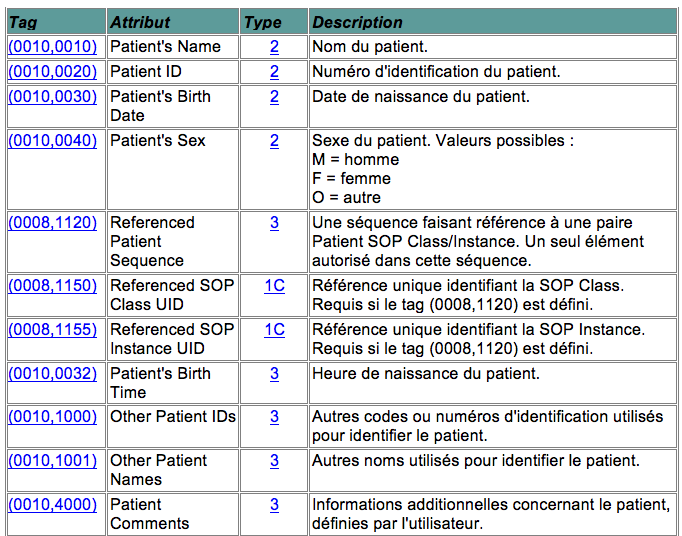
\includegraphics[width=.45\linewidth]{./figures/table.png}
	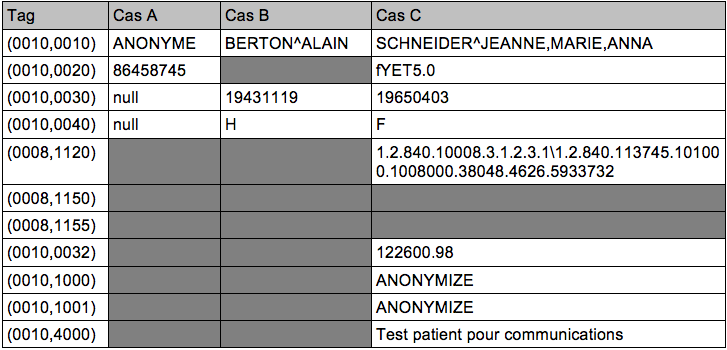
\includegraphics[width=.45\linewidth]{./figures/metadata-cases.png}
    
    Les cases gris\'ees indiquent un champ absent, \emph{null} un champ pr\'esent, mais vide.
}



\end{document}
